% !Mode:: "TeX:UTF-8"
\chapter{绪\quad 论}
\label{chap:introduction}
\section{引言}
{\normalsize 随着人类社会科学技术的进步,}文本与图像数据作为信息的载体呈指数爆炸式增长,人类进入大数据和人工智能时代。深度学习方法是最近计算机视觉与自然语言处理快速发展的基础。相位恢复为典型的非凸优化问题,有效的求解算法依赖图像先验的约束。如何将深度学习中的去噪算法作为高级图像先验引入相位恢复问题,构建高效的求解算法具有重要的实践应用价值。

\section{课题研究背景及意义}
相位恢复问题旨在通过非线性物理测量系统(散射介质成像或编码衍射成像模型)生成的衍射图案或强度值信息重构原始图像。相位恢复在应用物理学与工程领域得到了广泛的应用,主要包括计算生物学、X射线晶体学、光学、图像盲解卷积、天文成像和编码衍射成像\supercite{Jaganathan,Grohs,Tillmann,Candes,Gross,Baoshun}。在众多物理测量系统中,人们只能测量功率谱密度,即原始信号傅里叶变换或其他非线性变换模值的平方。例如,在光学仪器中,CCD照相机和感光片之类的检测装置不能测量光波的相位,而是测量光子通量。此外,在距成像平面足够远处,光学装置通过图像的傅里叶变换给出标量场\supercite{Metzler0}。因此,远场成像中光学装置基本上测量傅立叶变换的幅值或强度值,造成编码图像结构信息的相位丢失。如图\ref{fig:1-1}所示,它给出了图像Barbara和Pollen交换其傅里叶变换相位后的重构示意图。
\begin{figure}[!htbp]  
	\centering
	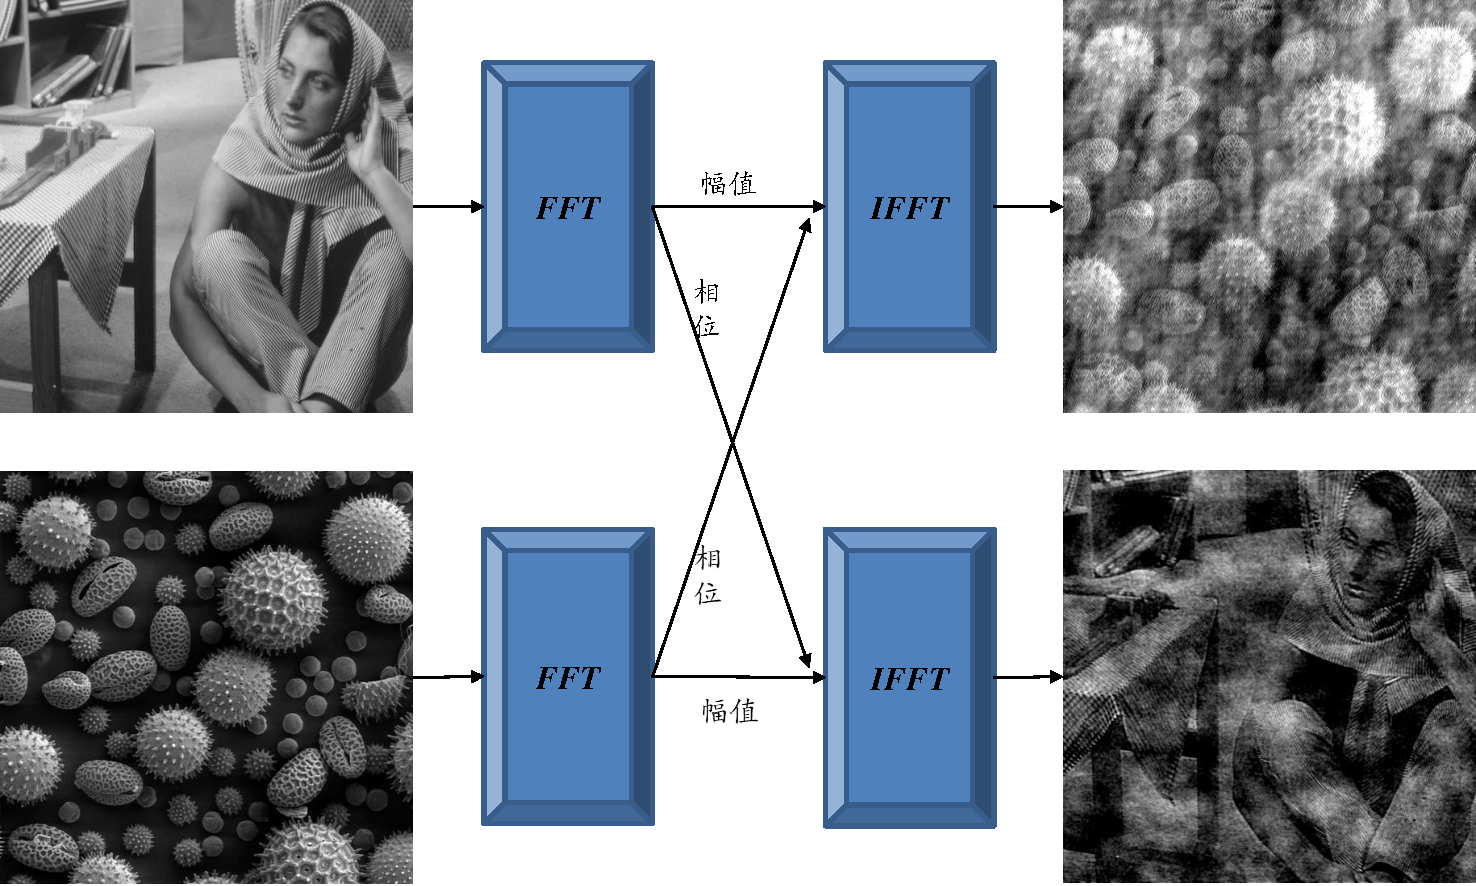
\includegraphics[width=0.8\linewidth]{1-1}
	\caption{Barbara与Pollen交换傅里叶相位后的重构示意图}\label{fig:1-1}
\end{figure}

图\ref{fig:1-1}中FFT表示傅里叶变换,IFFT表示傅里叶逆变换。从图\ref{fig:1-1}可以看出图像傅里叶变换的相位部分表征更多关于图像结构的信息。如何利用缺失相位的观测数据重构原始图像是图像重构领域的一大挑战。

站在优化的视角,相位恢复问题因非线性测量一般为非凸优化问题,其相位信息的缺失致使满足幅值非线性方程得解有无穷多个,即解空间非凸。较之凸优化问题,非凸优化问题在高维向量空间中存在多个局部候选解和鞍点,求解全局最优至少为NP(Non-deterministic Polynomial)难问题。为解决该不适定问题,现有算法通常利用图像的先验知识,包括非负性、非局部自相似性以及稀疏性等约束解空间\supercite{LiYin}。证明相位恢复算法的收敛性和收敛速度是非凸优化领域研究的难题\supercite{Hand,Jagatap,Tobias}。

深度学习在解决线性和非线性图像反问题方面取得了前所未有的成功\supercite{Ulyanov,Ulyanov,Mataev}。在图像去噪、超分辨率、图像修复、压缩感知和相位恢复等图像反问题中,基于深度卷积神经网络(Convolutional Neural Networks, CNN)的方法重构图像的质量和测试速度均优于传统的优化方法。深度生成先验已经替代了传统人工设计的图像先验,比如稀疏性,全变差,块匹配与三维滤波(Block-Matching and 3D Filtering,BM3D)、非局部自相似性等图像先验。然而深度生成先验受限于其对数据的敏感性,在面对无标签、仅有弱标签或者合成的伪标签数据时,深度生成先验的优势难以充分体现。如何将基于无监督学习的深度图像先验应用于相位恢复问题有待进一步研究。

\section{国内外研究现状}

\subsection{国内研究现状}
2012年,上海交通大学的文再文等人利用增广拉格朗日方向交替法(Augmented Lagrangian Alternating Direction Method,ADM)求解经典的图像相位恢复问题,指出了ADM算法与投影算法之间的联系,并与标准的相位恢复算法HIO(Hybrid Input-Output)、HPR(Hybrid Projection Reflection)和RAAR(Relaxed Averaged Alternating Reflection)在多幅测试图像上的性能进行比较,验证了该算法对参数的鲁棒性。

2017年,燕山大学的魏天姣等人将自然图像在梯度域下的稀疏性用于相位恢复。该算法将全变差正则项以目标函数求和的方式融合到基于支撑约束和幅值约束的相位恢复问题中,并利用ADMM算法对所提的非凸优化问题进行求解。

2018年,燕山大学的李颖等人结合图像在小波域的组稀疏性与图像在梯度域的稀疏性,面向编码衍射模型提出一种融合正交小波db10和sym4组稀疏性与全变差正则化的相位恢复算法\supercite{LiYin}。

2018年,燕山大学的石保顺等人提出了一种称为约束相位恢复的统一框架,将交替投影方法和正则化方法结合在一起。所提ConPR(Constrained Phase Retrieval)框架不仅可以从少量衍射图形中恢复高质量的图像,而且还不需要对参数进行微调。该方法将块匹配和三维滤波框架下的稀疏性纳入到所提出的ConPR框架中。优化问题由图像更新子问题和图像去噪子问题组成,之后依据数据保真项的上图概念求解数据保真项对应的优化子问题\supercite{Baoshun}。

2020年,北京理工大学的魏恺轩等人利用强化学习技术进行邻近算法迭代策略的深度展开,提出了一种免调参的即插即用邻近算法。该算法的关键部分是开发一个用于参数自动搜索的策略网络,可以通过混合无模型和基于模型的深度强化学习来有效地学习邻近算法的内部迭代参数,包括惩罚参数,降噪强度和终止时间。该算法用于解决核磁共振成像(Magnetic Resonance Imaging,MRI)和编码衍射成像问题,并且数值实验取得当前最佳(State of the Art,SOTA)的图像重构结果\supercite{Kaixuan}。

\subsection{国外研究现状}
2007年,加利福尼亚大学的Marchesini等人从交替投影策略的观点出发总结了ER、SF、HIO、DM、ASR、HPR、RAAR等算法,并应用最速下降法、共轭梯度法、最大-最小算法(Majorization Minimization,MM)求解关于衍射显微镜成像中的相位恢复问题。

2013年,斯坦福大学的Cand{\`e}s等人首次提出编码衍射模型来解决一维相位恢复问题。 Cand{\`e}s利用凸松弛技术:相位提升进行信号重构。该算法利用矩阵提升技术将相位恢复问题转化为低秩最小化问题。通过理论和实验证明它能从多个随机调制图案中准确地恢复相位信息,这些随机调制图案的采样数量为对数复杂度。但矩阵提升对于二维图像计算过于复杂,致使该算法应用受限\supercite{Candes}。

2015年,斯坦福大学的Cand{\`e}s等人提出了类似于梯度下降的WF(Wirtinger Flow)方法解决非凸形式的相位恢复问题,并以谱方法估计初始值。该算法允许从随机测量值中精确地恢复信号,具有拟线性收敛率。数值实验表明,在无噪情况下,该算法利用多个编码衍射图案能够完全重建原始图像,是近些年比较优秀的算法之一。随后,他们对WF算法进行了改进,提出了针对泊松噪声情况的TWF(Truncated Wirtinger Flow)算法。该算法在梯度计算时引入了截断机制,修正了梯度下降方向\supercite{Gross}。 

2016年,达姆施塔特工业大学的Tillmann等人提出了基于字典学习的相位恢复算法,该算法在字典未知的情况下,将待恢复图像假设为稀疏信号。在这一假设下,该算法联合重建被噪声污染的未知信号同时进行字典更新,使得估计的图像中的每一个图像块都可以被稀疏地表示。在理论上,Tillmann证明了该算法的收敛性\supercite{Tillmann}。

2018年,莱斯大学的Metzler提出prDeep算法用来解决散射介成像和转角成像中的相位恢复问题。该算法将去噪卷积神经网络DnCNN(Feed-forward Denoising Convolutional Neural Networks)嵌入RED正则化框架,利用FASTA(Fast Adaptive Shrinkage/Thresholding)算法进行求解。实验证明,该算法对泊松噪声具有鲁棒性并且能够处理各种测量矩阵模型\supercite{Metzler1}。

2019 年,美国东北大学的Hand提出了基于深度生成生先验的DPR(Deep Phase Retrieval)算法。该算法利用子梯度下降训练自编码神经网络,并依据损失函数的优化视图发现全局极小值的存在\supercite{Hand}。同年,Jagatap等人提出了基于深度图像先验(Deep Image Prior,DIP)的压缩相位恢复算法:Net-GD(Network Gradient Descent)与Net-PGD(Network Projected Gradient Descent)。数值实验结果表明,该算法在较低采样率的情况下重构图像质量优于基于稀疏先验的TVAL3、Lasso等压缩相位恢复算法。另外,在观测矩阵服从高斯分布并且满足RIP(Restricted Isometry Property)的假设下,他们证明了该算法的收敛性与最优采样复杂度的下界\supercite{Jagatap}。

\section{研究内容及结构安排}
上述国内外研究成果表明学者对实际工程应用中相位恢复算法研究的高度重视,并且取得了很多原创性成果,但也存在一些问题需要进一步攻克。本文重点研究该领域两个关键问题:散射介质成像与编码衍射成像中的相位恢复问题。散射介质成像系统如图\ref{fig:1-2}所示,相干光束照射观测目标经过空间光调制器(Spatial Light Modulator,SLM)生成衍射图案\supercite{Metzler0}。
\begin{figure}[!htbp]
	\setlength{\abovecaptionskip}{-0.02\linewidth}   
	\centering
	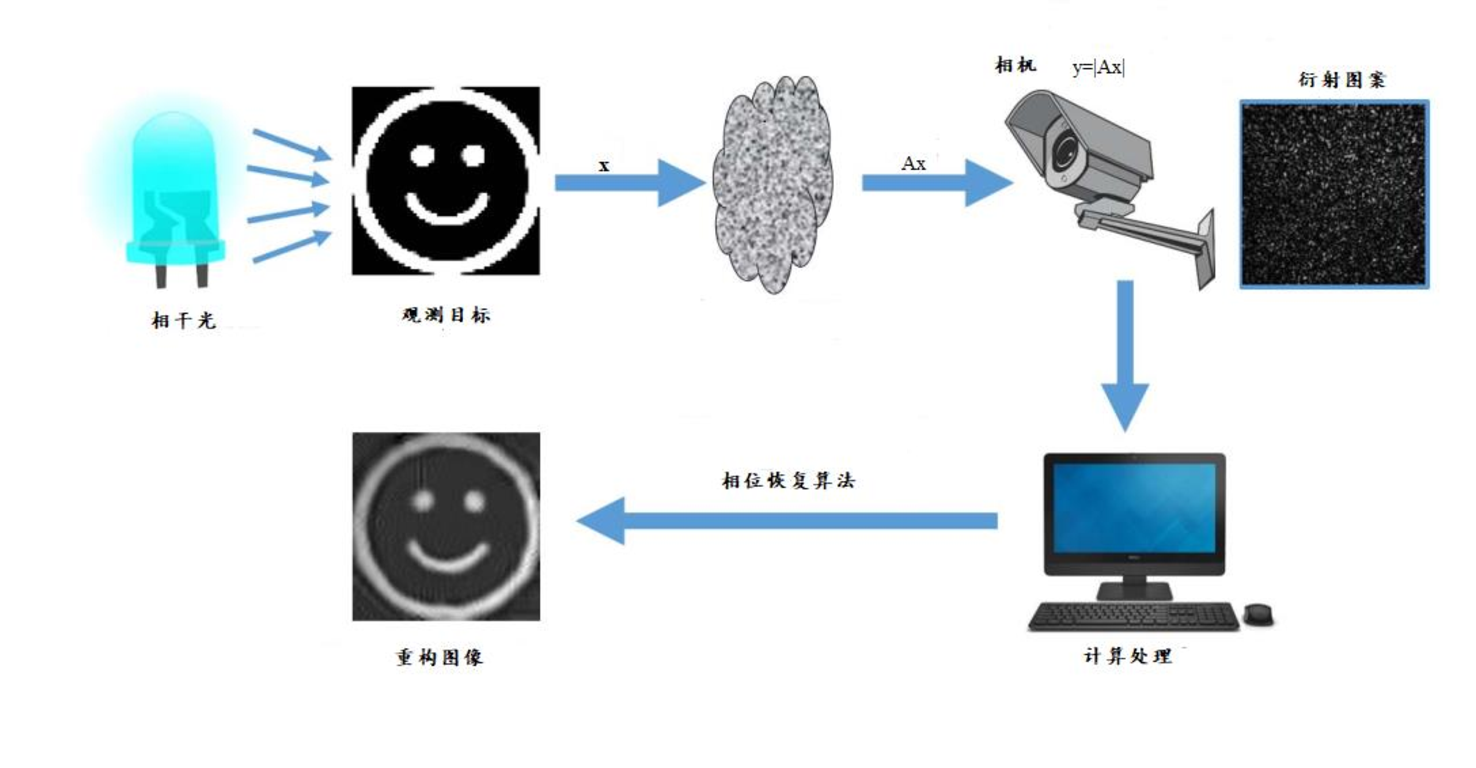
\includegraphics[width=0.8\linewidth]{1-2}
	\caption{散射介质成像装置示意图}\label{fig:1-2}
\end{figure}

编码衍射模型如图\ref{fig:1-3}所示,激光束照射待观测物体穿过相位板生成衍射图案\supercite{Candes}。二者唯一的的区别在于传输矩阵不同。为了解决上述问题,本文深入挖掘基于深度学习的去噪器和去噪正则化等高级图像先验,研究凸优化理论中的共识优化与共识方程、非凸优化理论中的基于梯度的一阶随机优化方法、基于无监督学习的深度图像先验等前沿技术构建了高效的相位恢复算法。本文主要研究内容包括如下几个方面:

(1)在编码衍射模型下,将编码衍射模型数据保真项的近邻算子与图像去噪算子作为共识方程的两个代理,提出了基于共识方程的编码衍射成像算法。在理论层面推广了文献\cite{Xiran}给出的收敛性假设条件。最后本文设计数值实验验证了该算法对含高斯和泊松噪声观测值的鲁棒性;

(2)在编码衍射模型下,依据编码衍射图案的可分离特征,提出了基于一阶随机优化的编码衍射成像算法。最后本文设计数值实验验证该算法在大规模编码衍射图案上的加速效果;

(3)在压缩相位恢复问题中,利用未训练神经网络捕获深度图像模式,并融合RED先验提出了基于深度图像先验融合RED正则项的压缩相位恢复算法。在欠采样的高斯观测矩阵下,本文设计数值实验验证该算法的重构性能以及对噪声的鲁棒性。
\begin{figure}[!hptb]  
	\centering
	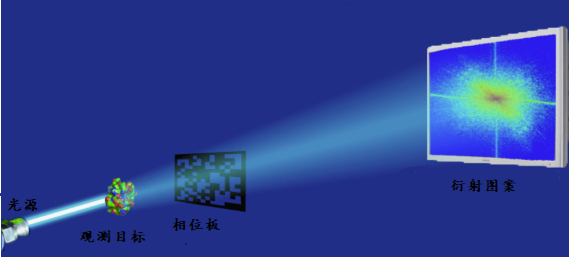
\includegraphics[width=0.6\linewidth]{1-3}
	\caption{编码衍射成像系统示意图}\label{fig:1-3}
\end{figure}

基于上述几节的研究与讨论,本文对基于非凸优化和深度学习的相位恢复算法进行了深入研究,本文的行文结构安排如下:

第\ref{chap:introduction}章,绪论。首先介绍了相位恢复问题的研究背景及其研究意义,其次总结了相位恢复的国内外研究现状,最后明确了本文的研究内容和组织结构。

第\ref{chap:theory}章,非凸优化与深度学习基本理论。首先阐述了非凸优化理论的基本问题和基本算法,其次表述了深度学习领域的基本网络架构和基于深度学习的图像去噪算法DnCNN与IRCNN(Image Restoration Convolutional Neural Networks)。

第\ref{chap:ce}章,基于共识方程的编码衍射成像算法。首先介绍了基于即插即用先验的PnP-ADMM和PnP-FBS算法以及基于RED先验的prDeep算法,其次推导了共识优化到共识方程的演化过程,最后提出了基于共识方程的编码衍射成像算法,在理论层面推广了文献\cite{Xiran}给出的收敛性假设条件。数值实验结果证明了在重构实图像时,该算法能较好的保留图像更多纹理与结构信息,具有明显的优势。

第\ref{chap:stochastic}章,基于一阶随机优化的编码衍射成像算法。首先分析了一阶随机优化算法,然后依据编码衍射图案的可分离结构提出了基于一阶随机优化的编码衍射成像法。数值实验结果表明了在编码衍射模型下,该算法可看作是第三章提出的TACE算法的加速版本,主要用于处理大规模编码衍射图案。

第\ref{chap:dip}章,基于深度图像先验融合RED正则项的压缩相位恢复算法。首先简述了深度图像先验的基本原理,然后提出了基于深度图像先验融合RED正则项的压缩相位恢复算法。该算法将显式的RED先验作为正则项添加到隐式的深度图像先验损失函数中,并利用ADMM算法进行求解。无噪与含高斯、泊松噪声的数值仿真实验证明了DPR-RED算法在欠采样率下完美重建图像的有效性以及对噪声的鲁棒性。

%第\ref{chap:chap-5}章则介绍了在文章内加入计算机程序源代码的方法。

%第\ref{chap:unit}章介绍输入数字和物理量的方法。

最后,对本文的研究工作进行了总结、归纳和分析,并指出了研究过程的不足之处,展望了下一步的研究内容。 